\documentclass[a4paper, 12pt]{article}

% --- 1. Gói lệnh cơ bản ---
\usepackage[english]{babel}
\usepackage[utf8]{inputenc}
\usepackage[T1]{fontenc} % Sửa lỗi font shape undefined
\usepackage{lmodern}
\usepackage{graphicx}
\usepackage{fancyhdr}
\usepackage{array} 
\usepackage{amsmath}
\usepackage{amsfonts}
\usepackage{amssymb}
\usepackage{bm}
\usepackage{float}

% --- 2. Cấu hình Header & Footer ---
\setlength{\headheight}{15pt}
\addtolength{\topmargin}{-3pt}
\pagestyle{fancy}
\fancyhf{}
\lhead{FPT School of Business \& Technology}
\cfoot{\thepage}
\rfoot{Group3-MSE23HN}
\renewcommand{\headrulewidth}{0.5pt}
\renewcommand{\footrulewidth}{0.5pt}

\begin{document}
	\sloppy
	
	% --- 3. TRANG TIÊU ĐỀ ---
	\begin{titlepage}
		\begin{center}
			
\includegraphics[scale=0.3]{Images/fpt.png} 
		\end{center}
		
		\center
		\vspace{0.5in}
		\textbf{\large MASTER THESIS PROPOSAL}
		\vspace{0.5in}
		
		\noindent\makebox[\linewidth]{\rule{\linewidth}{1.2pt}}
		\textbf{\large A Multimodal AI Agent Framework for Comprehensive Traffic Scene Understanding and Intelligent Control}
		\noindent\makebox[\linewidth]{\rule{\linewidth}{1.2pt}}
		
		\vspace{0.5in}
		
		\begin{minipage}{0.65\textwidth}
			\begin{flushleft}
				\textit{Students:} \\
				\vspace{0.1in}
				\begin{tabular}{|l|l|}
					\hline
					Ngo Vi Viet Anh & MSE13205 \\ \hline
					Trinh Thi Mai Huong & MSE13176 \\ \hline
					Nghiem Phan Thanh Tuan & MSE13189 \\ \hline
					Do Minh Hieu & MSE13172 \\ \hline
				\end{tabular}
			\end{flushleft}
		\end{minipage}
		\begin{minipage}{0.3\textwidth}
			\begin{flushright}
				\textit{Advisor:} \\
				Dr. Le Minh Duc \\
			\end{flushright}
		\end{minipage}
		
		\vspace{2in}
		\textbf{\large GRI501 - Group 3} \\
		\today
	\end{titlepage}
	
	% --- 4. ĐÁNH SỐ TRANG ---
	\pagenumbering{arabic}
	\setcounter{page}{2}
	\tableofcontents
	\newpage
	
	\section{Introduction}
	The digital transformation of urban mobility infrastructure has catalyzed significant advancements in autonomous driving and intelligent transportation systems. In the modern era, traditional computer vision methodologies have achieved substantial success in localized tasks, such as entity detection and vehicle classification \cite{nguyen2023object, ji2020action}. However, as the complexity of autonomous navigation increases, modern traffic management demands a profound understanding of behavioral patterns and spatio-temporal dependencies, transitioning from mere static object identification to high-level semantic reasoning \cite{mao2023gpt4, zheng2024llmits}.
	
	While current intelligent systems excel in structured, lane-based environments, they face severe limitations when deployed in highly heterogeneous conditions. Vietnam presents a unique and challenging scenario for these systems. Unlike structured Western traffic patterns, Vietnamese urban mobility is characterized by an extreme density of motorcycles, non-linear movement trajectories, and a systemic lack of rigid lane discipline \cite{ly2025enhancing, vo2021density}. Conventional retrieval methods, which rely on basic metadata or visual similarity, lack the semantic fidelity required to interpret complex safety-critical maneuvers, such as sudden lane cutting or opposite-direction travel in crowded intersections \cite{wang2021interaction, cao2023graphmatching}. 
	
	
	
	Consequently, the primary objective of this research proposal is to elucidate how unstructured traffic scenes can be accurately modeled and semantically interpreted. This study aims to propose a multimodal AI agent framework that synergizes Large Language Models, Knowledge Graphs, and Reinforcement Learning to resolve the ambiguity of mixed traffic and provide an intelligent, real-time traffic signal control mechanism.
	
	\section{Background}
	To establish a comprehensive foundation for this proposal, it is essential to examine the current state of research across four interconnected technological domains. This section outlines the existing methodologies, ongoing advancements, and the critical challenges that currently impede the deployment of autonomous systems in complex urban environments.
	\subsection{Unsupervised 3D Scene Reconstruction from Sparse LiDAR}
	Foundational to all semantic understanding and control is the geometric accuracy of the perceived environment. Current perception pipelines are heavily focused on transitioning from 2D visual data to rich 3D world models. A major research focus is reconstructing complete, physically-plausible 3D scenes from sparse LiDAR point clouds or monocular videos \cite{cao2023graphmatching}. Because acquiring densely annotated 3D data is prohibitively expensive, researchers are adopting unsupervised learning methodologies. These approaches attempt to fill in missing geometric points and resolve occlusions by enforcing physical constraints (such as gravity and surface smoothness) without relying on supervised ground-truth labels. The persistent difficulty here lies in maintaining geometric fidelity in highly chaotic environments, where the sheer density of dynamic obstacles (e.g., swarms of motorcycles) continuously occludes the underlying road infrastructure \cite{vo2021density, wang2021interaction}.
	
	\subsection{Semantic Lane and Road Marking Understanding for Traffic Decision Support}
	Current research in traffic scene perception is undergoing a paradigm shift from traditional pixel-level object detection to high-level semantic reasoning. Historically, models relied on convolutional neural networks to identify explicit physical boundaries and entities \cite{nguyen2023object}. However, modern autonomous frameworks increasingly utilize Large Language Models (LLMs) and Vision-Language Models (VLMs) to achieve human-like cognitive understanding of road topologies \cite{zheng2024llmits, fu2024drivelm}. Researchers are exploring techniques such as Chain of Thought (CoT) prompting to enable these models to deduce implicit rules and semantic lane structures, even when physical markings are degraded or absent \cite{wei2022cot}. Despite these advancements, a significant difficulty remains: these language models often struggle to maintain reasoning accuracy in highly unstructured environments where driving behaviors deviate from standardized rule sets, leading to unpredictable decision support outcomes \cite{tian2025query, wen2023dilu}.
	
	\subsection{Reinforcement Learning for Traffic Scene Retrieval and Reasoning}
	As traffic environments are increasingly modeled as dense spatio-temporal graphs (Road Scene Graphs), processing these massive data structures has emerged as a primary bottleneck \cite{roadscene2vec2024, li2022spatio}. The current methodology involves integrating Knowledge Graphs (KGs) with LLMs to ground the model's reasoning in factual traffic rules \cite{pan2024kgllm, yasunaga2021qagnn}. However, feeding entire scene graphs into an LLM frequently results in "Token Saturation" and "Context Rot," where the model loses focus due to information overload \cite{hong2025contextrot, zhang2026recursive}. To overcome this, the latest research trend introduces Reinforcement Learning (RL) to dynamically navigate and prune these graphs before the reasoning stage \cite{edge2024graphrag, hu2024rlrag}. Algorithms like Group Relative Policy Optimization (GRPO) are being tested to train agents that selectively retrieve only the most safety-critical relational paths \cite{tencent2025grpo, chen2025pathrag}. The core challenge in this domain is balancing the aggressive pruning of data with the preservation of critical semantic context, especially during multi-hop reasoning tasks \cite{song2025plan, jiang2024graphllm}.
	
	\subsection{LLM-Guided Agents for Traffic Light Management}
	In the realm of infrastructure control, there is a strong movement toward replacing heuristic, rule-based traffic signal controllers with AI-driven meta-controllers \cite{ly2025enhancing}. Current studies are developing LLM-based agents capable of proactively managing traffic lights by processing real-time multimodal inputs and reasoning about multi-objective outcomes, such as minimizing wait times while prioritizing emergency vehicles \cite{shao2024lmdrive, wang2024knowledgedriven}. These frameworks attempt to fuse reactive flow management with deliberative safety-critical reasoning \cite{wang2025vlmlight, schmidt2025tls}. The primary obstacle encountered in this field is the latency introduced by deep semantic reasoning. Ensuring that an LLM agent can process complex scene graphs and issue control commands within the strict real-time constraints of an active intersection remains a formidable technical hurdle.
	
	
	
	\subsection{Conclusion on the Current Landscape}
	Collectively, the current research landscape illustrates a clear trajectory toward integrating structural geometric perception with advanced cognitive reasoning. While individual domains have achieved significant milestones, they operate largely in isolation. The overarching problem is the computational friction that occurs when massive, unstructured environmental data is fed into reasoning engines. Existing models lack a cohesive mechanism to selectively retrieve and process only the most critical semantic information in real-time. This friction is severely exacerbated in unstructured traffic contexts. Addressing this systemic inefficiency forms the logical basis for the subsequent Literature Review, which will critically analyze the specific methodologies and limitations of the foundational studies in these areas.
	
	\subsection{Literature Review and Research Gap}
	To address the complexity of road scenes, the scientific community has explored several distinct technological domains. An inductive analysis of these areas reveals significant advancements along with persistent bottlenecks that justify the need for an integrated framework.
	
	\textbf{Road Scene Graph (RSG) Extractions.} The transition from pixel-level detection to topological representation has been spearheaded by frameworks like \textit{RoadScene2Vec}, which utilize spatio-temporal graphs to capture vehicle trajectories and relationships \cite{roadscene2vec2024, li2022spatio}. These methods provide a structured foundation for scene understanding. However, most existing RSG models are optimized for structured environments, failing to capture the stochastic nature of heterogeneous traffic in Vietnam \cite{tian2025query, wen2023dilu}. There is a clear need for a perception pipeline that translates unstructured local videos into standardized graphs without losing critical semantic details.
	
	\textbf{LLM and MLLM for Scene Understanding.} Large Language Models (LLM) and Vision-Language Models (VLM) have demonstrated unprecedented capacity for common-sense reasoning and planning in autonomous contexts \cite{wang2025vlmlight, fu2024drivelm}. Despite their potential, LLMs suffer from "Token Saturation" and "Context Rot" when processing dense, raw scene graphs \cite{fan2025minirag, zhang2026recursive, hong2025contextrot}. Feeding an entire graph into an LLM often leads to prohibitive computational latency and reasoning failures due to information redundancy.
	
	\textbf{Knowledge Graph (KG) Integration.} To ground LLM reasoning in factual truth, researchers have integrated Knowledge Graphs to encode traffic rules and ontologies \cite{morignot2014ontology, pan2024kgllm}. These structured knowledge bases improve interpretability but often remain static and struggle to adapt to rapidly changing road scenes. Furthermore, there is a lack of specialized ontologies that incorporate the specific behavioral nuances of mixed traffic scenarios prevalent in Southeast Asia.
	
	\textbf{Reinforcement Learning (RL) for Guided Retrieval.} Recent breakthroughs in reinforcement learning, such as Group Relative Policy Optimization (GRPO), have enabled models to optimize retrieval processes through adaptive scheduling \cite{song2025plan, tencent2025grpo}. RL has shown promise in pruning redundant paths in graph-based retrieval \cite{chen2025pathrag}. However, its application specifically for navigating road scene graphs to optimize semantic retrieval remains largely unexplored.
	
	\textbf{Synthesis and Research Gap.} By synthesizing these domains, a critical research gap is identified: there is no framework that effectively combines the structural fidelity of RSGs, the rich domain knowledge of KGs, and the adaptive navigation of RL to solve the problem of semantic retrieval in heterogeneous traffic. Existing methods either possess the data but lack reasoning efficiency, or possess reasoning power but are overwhelmed by data volume. %dẫn dắt\This research bridges this gap by proposing an RL-guided reasoning layer over a specialized Knowledge Graph, specifically calibrated for the complexity of Vietnam urban environments.
	
	
	
	\subsection{Research Objectives}
	The primary goal of this research is to develop an integrated framework that utilizes reinforcement learning to guide semantic reasoning over road scene knowledge graphs \cite{song2025plan, hu2024rlrag}. The core objectives are as follows:
	\begin{itemize}
		\item To engineer an automated pipeline that transforms raw Vietnam driving videos into standardized RSGs \cite{roadscene2vec2024, tian2025query}.
		\item To transform these preliminary graphs into structured Knowledge Graphs that incorporate local traffic behaviors and rules \cite{morignot2014ontology}.
		\item To design a reinforcement learning policy capable of identifying optimal sub-graphs for user queries with minimal computational overhead \cite{tencent2025grpo}.
	\end{itemize}
	
	The study addresses several fundamental questions:
	\begin{enumerate}
		\item Can an RL-guided agent significantly reduce token consumption while maintaining high reasoning accuracy in mixed traffic scenarios \cite{jiang2024graphllm}?
		\item To what extent does local traffic ontology integration improve the semantic retrieval of safety-critical events \cite{wei2022cot}?
		\item How can the framework maintain low latency during multi-hop reasoning over dense traffic graphs \cite{song2025plan, zhang2026recursive}?
	\end{enumerate}
	
	\subsection{Thesis Contributions}
	This research introduces a specialized Knowledge Graph architecture designed for the complexities of heterogeneous mixed traffic in Vietnam. It presents a novel retrieval mechanism guided by reinforcement learning, which optimizes the token consumption of language models by selecting only the most relevant knowledge paths for reasoning \cite{song2025plan, chen2025pathrag}. Additionally, the study provides a newly processed dataset of traffic scene graphs derived from real world driving videos, serving as an empirical resource for future investigations into semantic traffic understanding.
	
	\subsection{Thesis Scope and Limitations}
	The scope of this research is strictly bounded by daytime urban traffic scenarios within Vietnam to ensure high ecological validity \cite{vo2021density, ly2025enhancing}. The framework prioritizes reasoning efficiency over hardware level sensor fusion or real time vehicle control. While incorporating safety critical recognition for signs and signals \cite{schmidt2025tls}, it does not provide autonomous driving commands. Reasoning capabilities are delimited by the predefined ontology of the Knowledge Graph and the capacity of the selected language models. Environmental factors such as extreme weather or nighttime lighting are considered outside the primary scope of this evaluation.
	
	% ==========================================
	% 2. PROPOSED METHODOLOGY AND THEORETICAL FRAMEWORK
	% ==========================================
	\section{Methodology and Theoretical Framework}
	
	This section provides a rigorous exposition of the proposed technical framework. The methodology is designed as an end to end pipeline that transitions from raw geometric perception to high level semantic reasoning and proactive control. The framework is grounded in the principles of unsupervised learning, graph theory, and reinforcement learning.
	
	\subsection{Overall System Architecture and Pipeline Integration}
	The proposed system architecture is conceptualized as a hierarchical synergy of four primary modules, each designed to address a specific bottleneck in traffic scene understanding. The integration is governed by a unified data flow that ensures the preservation of semantic fidelity from perception to action.
	
	\begin{enumerate}
		\item \textbf{Geometric Reconstruction Layer:} This layer addresses the inherent sparsity of LiDAR point clouds. It utilizes unsupervised 3D reconstruction techniques to generate physically plausible environments, filling gaps caused by occlusions and sensor limitations \cite{roadscene2vec2024, li2022spatio}.
		\item \textbf{Semantic Interpretation Layer:} Following the reconstruction, a Large Language Model (LLM) acts as a semantic lifter. This layer extracts behavioral rules and traffic ontologies from the dense 3D scenes, specifically focusing on the non linear movement patterns prevalent in Vietnam \cite{tian2025query, wang2025vlmlight}.
		\item \textbf{Reasoning and Retrieval Layer:} These semantic insights are encoded into a Knowledge Graph (KG). A Reinforcement Learning (RL) agent is deployed to guide the reasoning process, identifying optimal knowledge paths for query resolution while mitigating the token saturation phenomenon \cite{song2025plan, tencent2025grpo, chen2025pathrag}.
		\item \textbf{Proactive Control Layer:} The final module utilizes the reasoned sub graphs to drive an LLM based traffic light management agent, optimizing signal phasing through a dual branch reasoning architecture \cite{wang2025vlmlight, schmidt2025tls}.
	\end{enumerate}
	\begin{figure}[H]
		\centering
		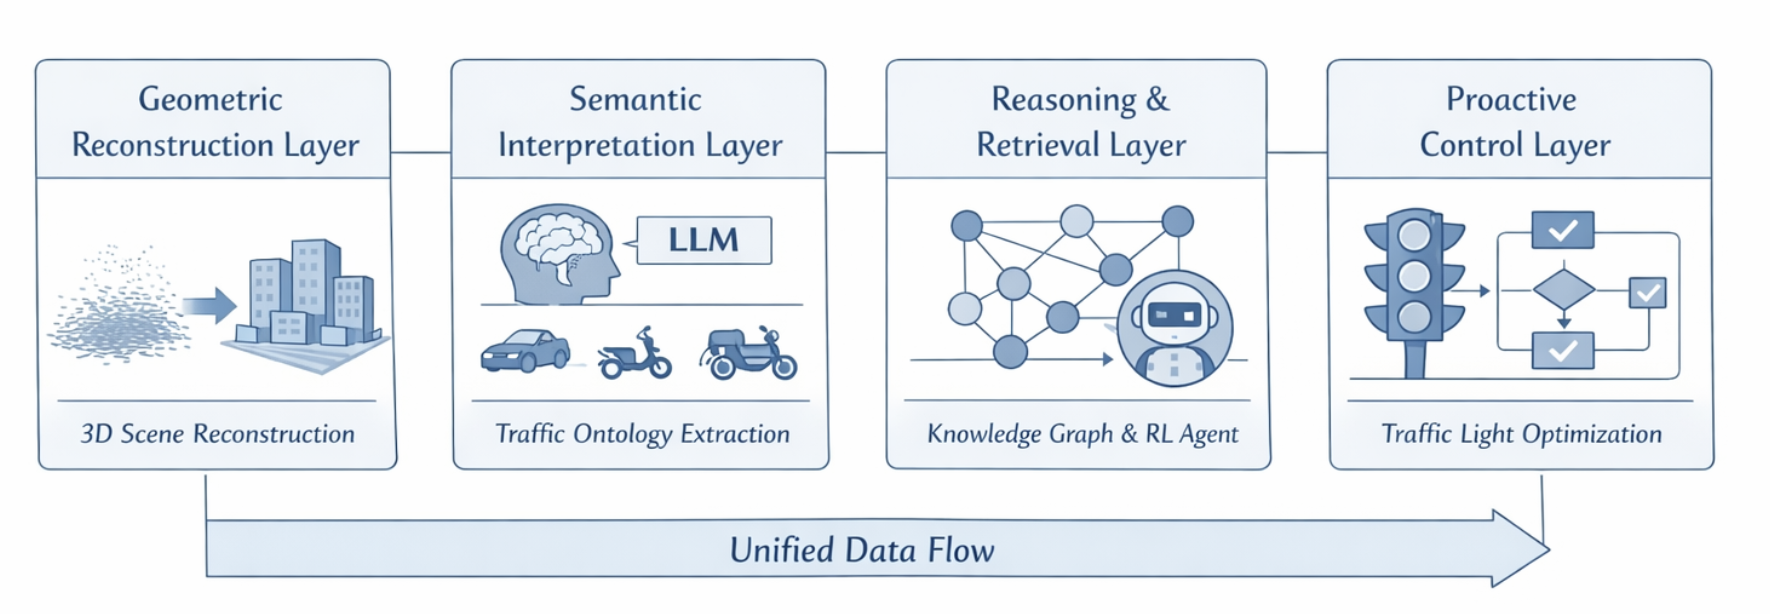
\includegraphics[width=1.0\textwidth]{Images/1.png}
		\caption{An integrated traffic intelligence framework showing perception, reasoning, and control modules}
		\label{fig:1}\
	\end{figure}
	
	
	\subsection{Unsupervised 3D Scene Reconstruction via Pseudo-LiDAR Generation}
	The foundational pillar of the perception pipeline is the reconstruction of a physically consistent 3D environment from monocular video sequences. Given the prevalence of motorcycles and unstructured movement in Vietnam, this module transforms raw 2D visual data into a 3D spatial representation to facilitate high level reasoning.
	
	\subsubsection{Theoretical Background and Problem Formulation}
	Let $\mathcal{I} = \{I_1, I_2, ..., I_T\}$ be a sequence of video frames captured from an urban Vietnam environment. The objective is to estimate the depth map $D_t$ for each frame to generate a Pseudo-LiDAR point cloud $\mathcal{P}_t \in \mathbb{R}^{N \times 3}$. Due to environmental occlusions and the absence of active depth sensors (LiDAR), $\mathcal{P}_t$ initially lacks structural completeness. 
	
	The task is formulated as finding a mapping function $\Phi: \mathcal{P}_t \rightarrow \mathcal{S}$ that produces a dense, physically plausible scene $\mathcal{S}$. In an unsupervised context, we leverage the principle of Geometric Consistency, assuming that road structures follow surface smoothness and structural symmetry invariants \cite{roadscene2vec2024, li2022spatio}.
	
	\subsubsection{Unsupervised Completion Methodology}
	To fill the missing regions without supervised labels, the framework utilizes a generative approach based on voxelized spatial probability. The reconstruction process aims to minimize a multi objective loss function $\mathcal{L}_{total}$:
	\begin{equation}
		\mathcal{L}_{total} = \mathcal{L}_{CD}(\mathcal{P}, \hat{\mathcal{S}}) + \lambda_1 \mathcal{L}_{smooth}(\hat{\mathcal{S}}) + \lambda_2 \mathcal{L}_{phys}(\hat{\mathcal{S}})
	\end{equation}
	Where $\mathcal{L}_{CD}$ is the Chamfer Distance ensuring fidelity to observed points, $\mathcal{L}_{smooth}$ penalizes abrupt surface discontinuities, and $\mathcal{L}_{phys}$ enforces gravity and non overlapping constraints \cite{ji2020action}. This ensures that even with sparse monocular inputs, the resulting 3D world model is structurally sound for semantic interpretation.
	
	\subsubsection{Implementation Pipeline}
	The reconstruction pipeline operates through three distinct stages. First, the \textbf{Structural Analysis} stage identifies low density regions in the voxel grid $\mathcal{V}$ that likely correspond to occluded surfaces. Second, the \textbf{Iterative Latent Filling} stage utilizes a generative network trained on structural priors (e.g., road planes, vertical walls) to predict the occupancy of the identified gaps. Third, the \textbf{Refinement Layer} applies temporal consistency checks across successive video frames from the Vietnam driving tour dataset, ensuring that the reconstructed scene remains stable over time and across different perspectives \cite{roadscene2vec2024, vo2021density}. This process results in a high fidelity 3D world model that serves as the basis for semantic lane understanding.
	\subsection{Semantic Lane and Road Marking Understanding via LLM Logic}
	The second module of the framework performs semantic lifting, transforming the reconstructed 3D geometric environment into a rule based behavioral model. This is essential for interpreting the unstructured nature of traffic in Vietnam, where formal lane boundaries are often secondary to informal driving protocols.
	
	\subsubsection{Semantic Mapping and Ontology Formulation}
	Let $\mathcal{S}$ be the dense 3D scene reconstructed in the previous stage. The system defines a semantic mapping function $\Psi: \mathcal{S} \times \mathcal{K}_{rules} \rightarrow \mathcal{G}_{enriched}$, where $\mathcal{K}_{rules}$ represents the domain knowledge of local traffic laws and $\mathcal{G}_{enriched}$ is the resultant semantic graph.
	
	The Large Language Model (LLM) is utilized as a zero shot semantic interpreter. Unlike traditional heuristic classifiers, the LLM processes a multimodal prompt consisting of the projected 2D road topology and textual descriptions of entity trajectories. The model employs Chain of Thought (CoT) prompting to deduce implicit road structures \cite{wei2022cot}. For instance, given a high density of motorcycles moving in parallel, the LLM infers a virtual motorcycle lane $\mathcal{L}_{motor}$ even in the absence of physical markings.
	
	\subsubsection{Theoretical Foundation: Semantic Predicate Extraction}
	\begin{figure}[H]
		\centering
		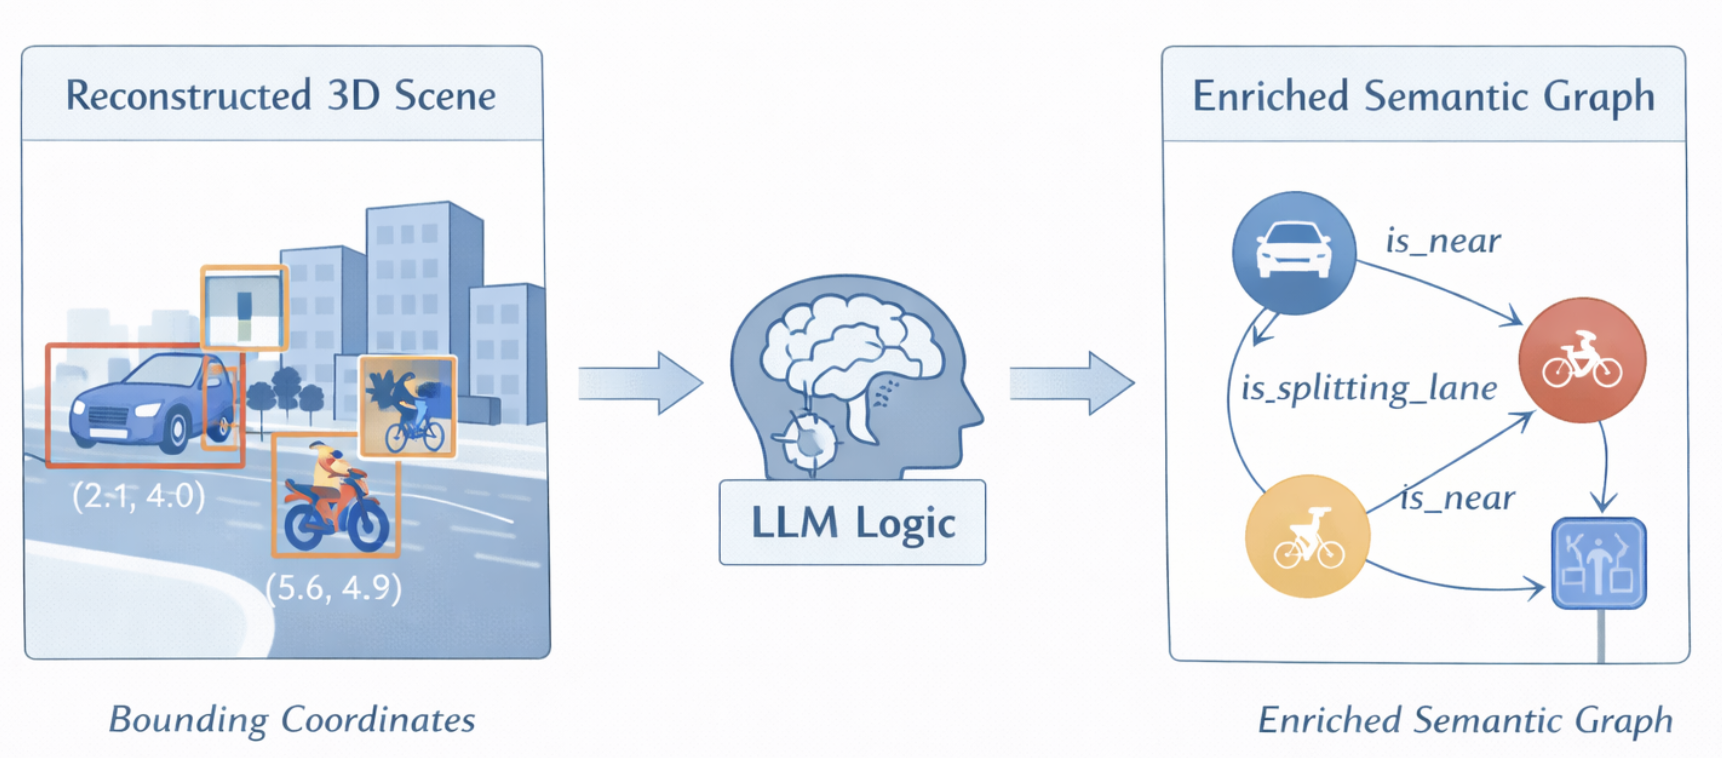
\includegraphics[width=0.9\textwidth]{Images/3.png}
		\caption{Conceptual workflow of semantic lifting: The LLM acts as an interpreter to transform geometric coordinates into logical predicates and behavioral ontologies.}
		\label{fig:3}
	\end{figure}
	The LLM extracts a set of semantic predicates $\mathcal{Q} = \{q_1, q_2, ..., q_m\}$ that define the state of the road. Each predicate $q$ represents a logical relationship:
	\begin{equation}
		q = \text{Relationship}(Entity_i, Entity_j, Context)
	\end{equation}
	Examples include $q_{yield}(bus, motorcycle)$ or $q_{lane\_splitting}(motorcycle, car)$. By encoding these behaviors into high level predicates, the framework ensures that the subsequent reasoning layer operates on human understandable logic rather than raw coordinate data \cite{tian2025query, morignot2014ontology}.
	
	\subsection{RL Guided Semantic Retrieval and Reasoning over Knowledge Graphs}
	The core of the reasoning mechanism is a dynamic navigation policy that operates over a Knowledge Graph (KG). This module solves the bottleneck of information redundancy and token saturation in Large Language Models \cite{fan2025minirag, zhang2026recursive}.
	
	\subsubsection{Markov Decision Process (MDP) for Graph Navigation}
	The retrieval process is formulated as an MDP defined by the quintuple $(\mathcal{S}, \mathcal{A}, \mathcal{P}, \mathcal{R}, \gamma)$.
	\begin{itemize}
		\item \textbf{State Space ($\mathcal{S}$):} At time step $t$, the state $s_t$ is a representation of the query embedding $e_q$, the current node $v_t \in \mathcal{V}_{KG}$, and the history of the traversed path $h_t = (v_0, e_0, v_1, ..., v_t)$.
		\item \textbf{Action Space ($\mathcal{A}$):} The action $a_t$ corresponds to selecting an outgoing edge $e \in \mathcal{E}_{v_t}$ to transition to a neighboring node $v_{t+1}$ or invoking a termination action to stop the search \cite{song2025plan, chen2025pathrag}.
		\item \textbf{Transition Probability ($\mathcal{P}$):} In a deterministic graph environment, $\mathcal{P}(s_{t+1}|s_t, a_t) = 1$ if the action leads to a valid adjacent node.
		\item \textbf{Reward Function ($\mathcal{R}$):} The agent is optimized using a reward function that balances semantic relevance and efficiency:
		\begin{equation}
			\mathcal{R}(s_t, a_t) = \alpha \cdot \text{Sim}(v_{t+1}, e_q) - \beta \cdot \text{Cost}(v_{t+1}) + \mathbb{I}_{answer} \cdot \Omega
		\end{equation}
		
		\begin{figure}[H]
			\centering
			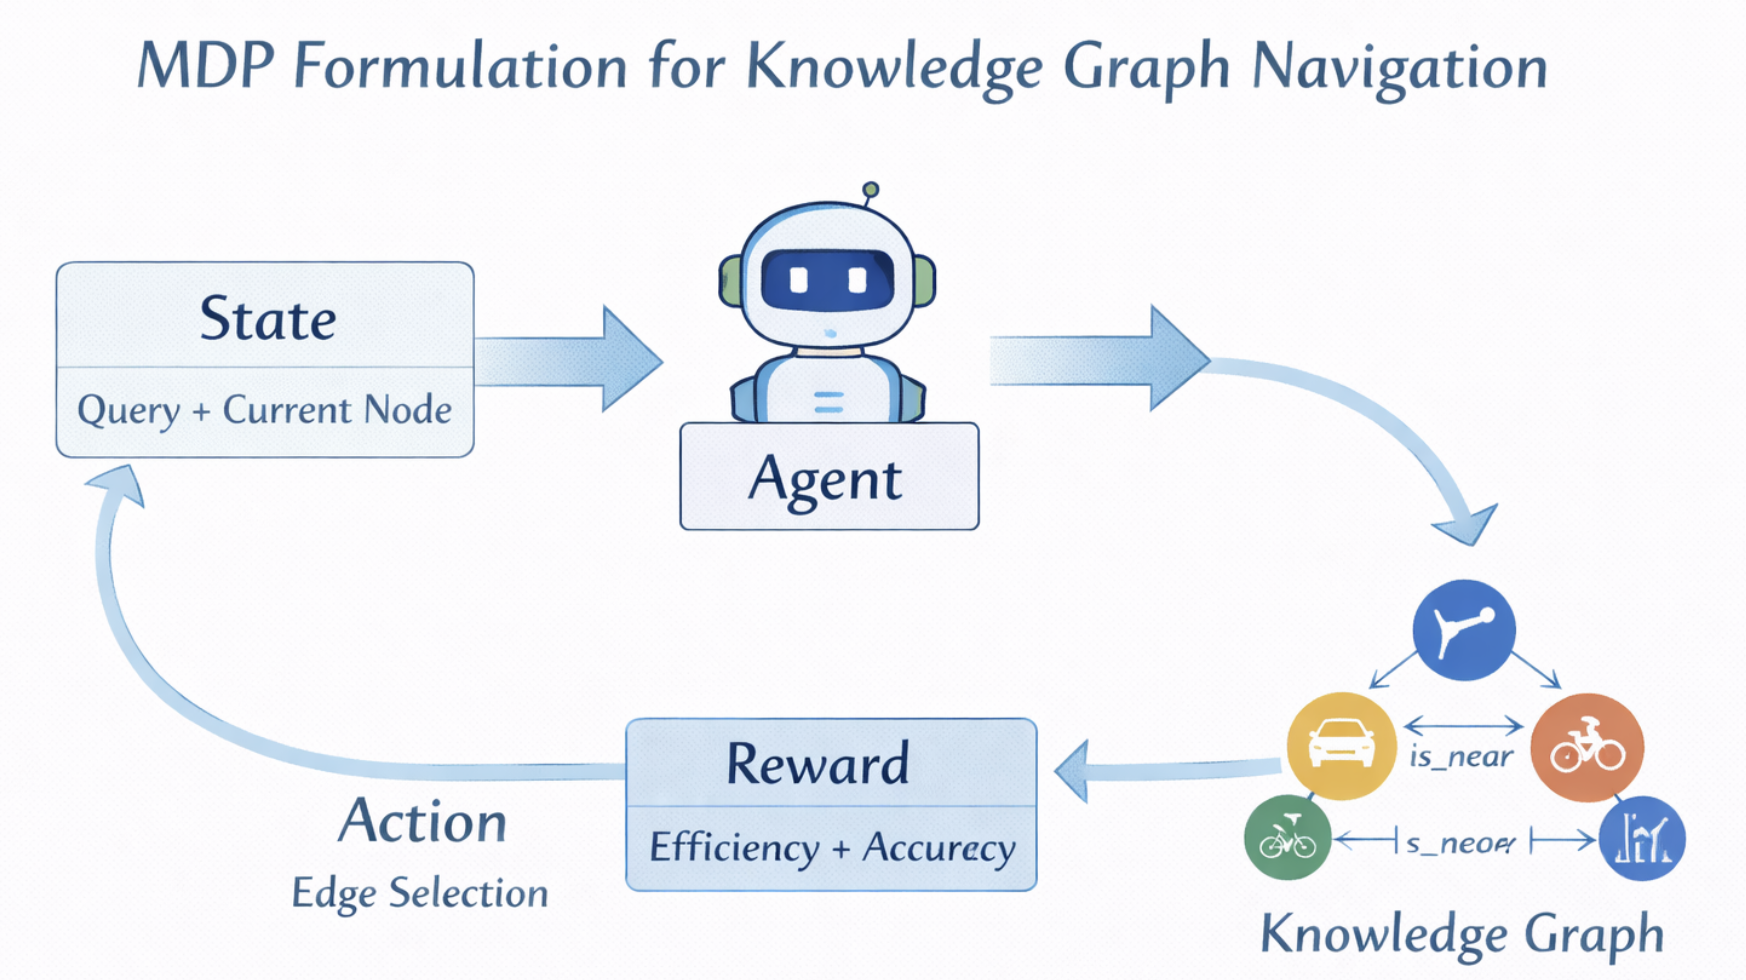
\includegraphics[width=0.9\textwidth]{Images/4.png}
			\caption{MDP Formulation for Knowledge Graph Navigation.}
			\label{fig:4}
		\end{figure}
		Where $\text{Sim}$ measures the cosine similarity between the node and the query, $\text{Cost}$ penalizes the token count of the node, and $\Omega$ is a terminal reward for reaching a node that answers the query.
	\end{itemize}
	
	
	
	\bibliography{sources}
	\bibliographystyle{IEEEtran}
\end{document}
